\ExerciseChapter{广义线性模型概述}

\label{chapter:1}

\par\addvspace{8pt}\noindent\begin{minipage}{\linewidth}

\section{作业题}

\subsection{简答题}

\Question{F1-1}{标准化、共线性与正态性诊断}

原反馈中的问题一并保留，供纠错练习：

\begin{enumerate}
\def\labelenumi{\arabic{enumi}.}
\tightlist
\item
  比较影响大小时为什么要标准化？标准化前后的 \(\beta\) 如何解释？
\item
  什么是复相关系数？
\item
  除决定系数外，如何用残差和交叉验证评价模型？
\item
  ``考虑到变量间的强相关性，对去除 LEP 或去除 BMI 进行了相同的回归分析''，意义何在？
\item
  ``正态性进行 K--S 检验，结果 \(P<0.001\)，说明 \(Y\) 的分布为连续型变量的正态分布''，这句话有何错误？\(H_0\) 是什么？
\end{enumerate}


\worklines{3}

\end{minipage}\par\vspace{5pt}

\par\addvspace{8pt}\noindent\begin{minipage}{\linewidth}

\subsection{数据分析题}

\Question{H1-1}{脂联素水平的影响因素}

为了研究有关糖尿病患者体内脂联素水平的影响因素，某医师测定了30名患者的体重指数 BMI（kg/m\(^2\)）、病程 DY（年）、瘦素 LEP（ng/mL）、空腹血糖 FPG（mmol/L）及脂联素 ADI（ng/mL）水平，数据如表11所示（数据文件：glmdata1）。\textbf{共8分。}

\begin{center}\small
\begin{tabular}{rrrrr@{\hspace{5mm}}rrrrr}
\toprule
BMI & DY & LEP & FPG & ADI & BMI & DY & LEP & FPG & ADI\\
\midrule
24.22 & 10.00 & 5.75 & 13.60 & 29.36 & 24.14 & 5.00 & 10.21 & 7.40 & 16.01\\
24.22 & 3.00 & 9.32 & 6.20 & 14.31 & 26.45 & 4.00 & 19.31 & 5.10 & 19.03\\
19.03 & 15.00 & 2.50 & 11.10 & 26.08 & 25.22 & 2.30 & 8.65 & 7.60 & 17.46\\
23.39 & 3.00 & 5.66 & 9.70 & 19.62 & 27.22 & 3.00 & 8.54 & 8.60 & 20.36\\
19.49 & 4.00 & 2.83 & 7.30 & 42.82 & 25.93 & 6.00 & 7.21 & 8.90 & 15.92\\
24.38 & 6.00 & 6.86 & 7.30 & 22.76 & 26.99 & 12.00 & 8.75 & 7.00 & 15.34\\
19.03 & 2.90 & 3.22 & 7.70 & 31.00 & 25.71 & 7.00 & 13.07 & 13.50 & 8.05\\
21.11 & 9.00 & 4.90 & 6.00 & 17.28 & 28.41 & 4.00 & 8.90 & 13.50 & 12.31\\
23.32 & 5.00 & 3.54 & 6.70 & 30.25 & 26.39 & 4.00 & 23.26 & 8.20 & 5.59\\
24.34 & 2.00 & 4.51 & 7.20 & 24.28 & 28.73 & 10.00 & 19.05 & 6.90 & 8.59\\
23.82 & 8.00 & 8.47 & 9.10 & 18.94 & 27.46 & 16.00 & 19.44 & 6.50 & 8.89\\
22.86 & 20.00 & 9.92 & 8.10 & 16.08 & 27.99 & 10.00 & 17.33 & 6.10 & 14.10\\
24.49 & 12.00 & 6.01 & 7.00 & 29.50 & 28.41 & 2.00 & 14.59 & 6.80 & 11.74\\
23.37 & 6.00 & 4.31 & 6.30 & 25.64 & 30.69 & 1.50 & 22.06 & 8.10 & 5.18\\
20.81 & 7.00 & 3.46 & 7.10 & 32.26 & 29.39 & 3.00 & 20.56 & 7.50 & 6.12\\
\bottomrule\end{tabular}\end{center}

\begin{enumerate}
\def\labelenumi{\arabic{enumi}.}
\tightlist
\item
  如何定量描述脂联素与各个影响因素之间的关系？
\item
  哪些因素对脂联素的影响具有统计学意义？
\item
  对脂联素影响最大的因素是谁？
\item
  如何评价模型拟合效果？
\item
  采用广义线性模型分析时，如何定义其因变量的分布和连接函数？
\item
  可以采用哪些方法进行参数估计？
\end{enumerate}


\worklines{3}

\end{minipage}\par\vspace{5pt}

\par\addvspace{8pt}\noindent\begin{minipage}{\linewidth}

\subsection{文献分析题}

\Question{H1-2}{肥胖与脑结构：文献分析}

阅读 Dekkers IA, Jansen PR, Lamb HJ. \emph{Obesity, Brain Volume, and White Matter Microstructure at MRI: A Cross-sectional UK Biobank Study}. Radiology. 2019;291(3):763--771。\textbf{共2分。}

\begin{enumerate}
\def\labelenumi{\arabic{enumi}.}
\tightlist
\item
  请阐述该研究的研究设计及分析思路。（1分）
\item
  总脑容量、皮质下灰质体积分别与 Total body fat（TBF）有何关系（Table 3/4）？（1分）
\end{enumerate}

\begin{center}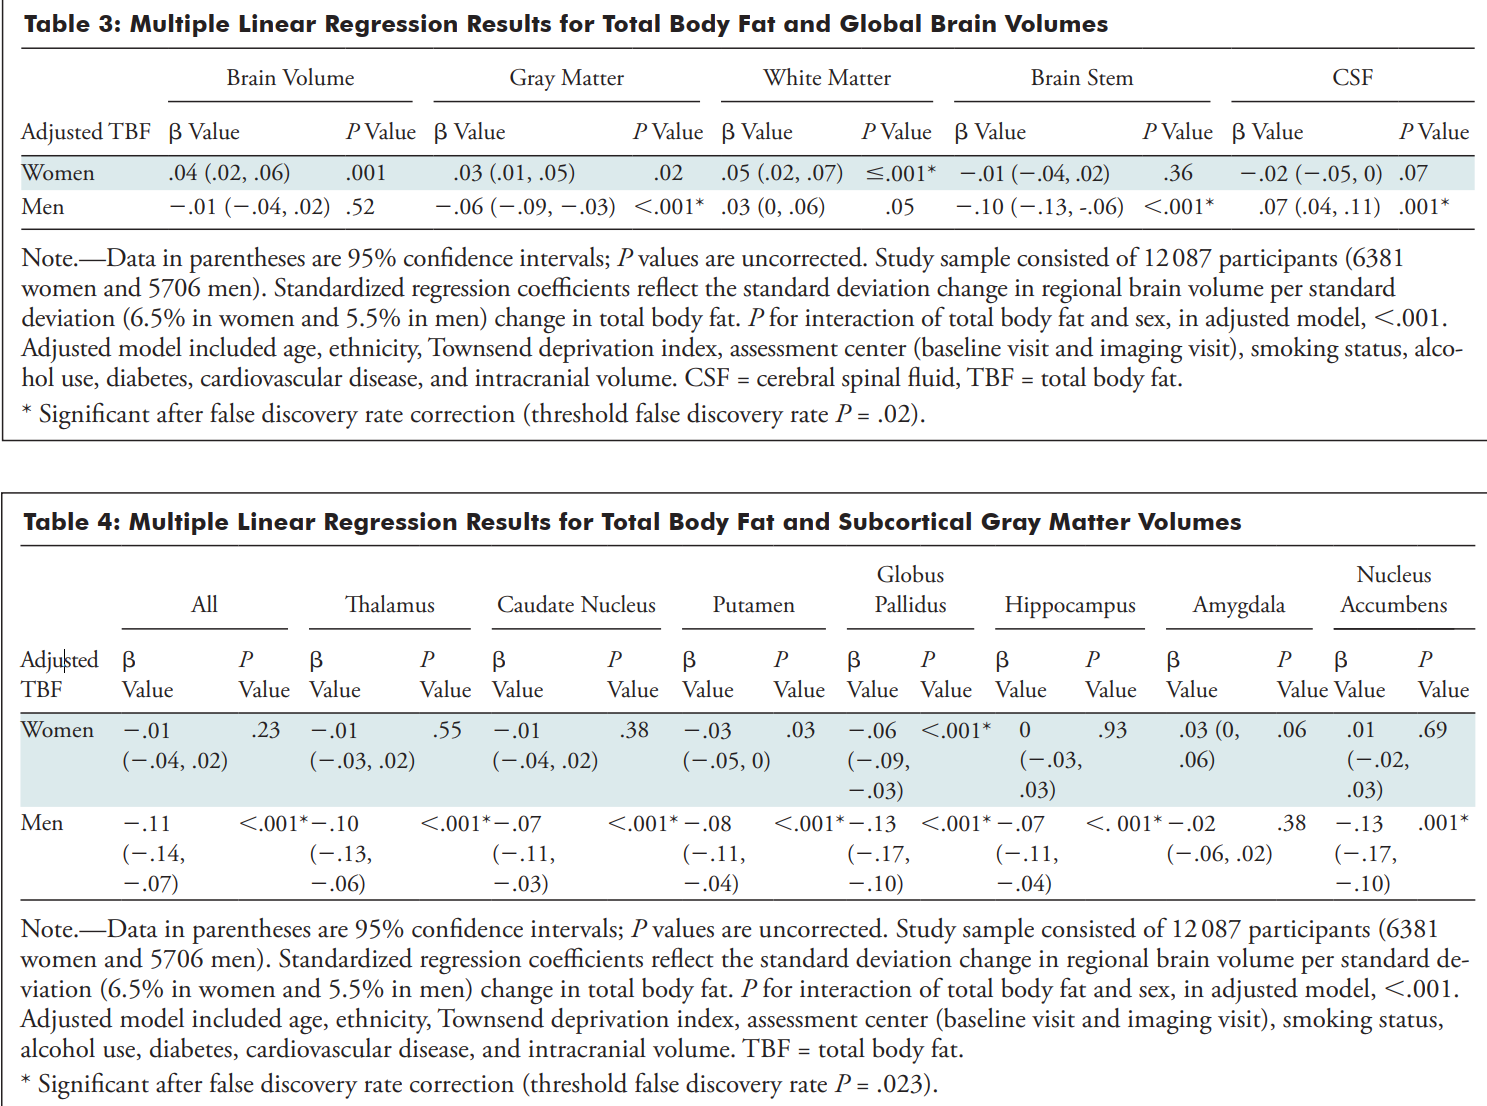
\includegraphics[width=\linewidth]{assets/brain_tables.png}\end{center}


\worklines{3}

\end{minipage}\par\vspace{5pt}

\par\addvspace{8pt}\noindent\begin{minipage}{\linewidth}

\section{往年题}

\subsection{单项选择题}

\Question{R24-M1}{自变量缩放与回归系数}

在含截距的多重线性回归中，将每个自变量 \(X_j\) 改写为 \(X_j^*=cX_j\)，其中 \(c>0\)。重新拟合后，偏回归系数与标准化偏回归系数如何变化？


\begin{choices}

\item 偏回归系数乘以 \(c\)，标准化偏回归系数不变。

\item 偏回归系数除以 \(c\)，标准化偏回归系数不变。

\item 二者均除以 \(c\)。

\item 二者均保持不变。

\item 偏回归系数不变，标准化偏回归系数乘以 \(c\)。

\end{choices}

\end{minipage}\par\vspace{5pt}

\par\addvspace{8pt}\noindent\begin{minipage}{\linewidth}

\Question{R24-M2}{复相关系数等于1}

在含截距且总平方和非零的多重线性回归中，复相关系数为1，以下哪项成立？


\begin{choices}

\item \(SS_{\text{残差}}=SS_{\text{总}}\)。

\item \(SS_{\text{回归}}=SS_{\text{总}}\)。

\item \(MS_{\text{残差}}=MS_{\text{总}}\)。

\item \(SS_{\text{回归}}=0\)。

\item \(SS_{\text{残差}}<0\)。

\end{choices}

\end{minipage}\par\vspace{5pt}

\par\addvspace{8pt}\noindent\begin{minipage}{\linewidth}

\Question{R24-M11}{连接函数的作用对象}

广义线性模型中，连接函数 \(g\) 通常将哪一项与线性预测子 \(X_i^T\beta\) 联系起来？


\begin{choices}

\item 每一个观测值 \(Y_i\) 本身。

\item 条件均值 \(\mu_i=E(Y_i\mid X_i)\)。

\item 每一个残差的平方。

\item 所有自变量的算术均数。

\item 回归系数的样本方差。

\end{choices}

\end{minipage}\par\vspace{5pt}

\par\addvspace{8pt}\noindent\begin{minipage}{\linewidth}

\subsection{名词解释}

\Question{R24-D1}{连接函数}

解释：连接函数。


\worklines{1}

\end{minipage}\par\vspace{5pt}

\par\addvspace{8pt}\noindent\begin{minipage}{\linewidth}

\Question{R24-D2}{拟合优度检验}

解释：拟合优度检验。


\worklines{1}

\end{minipage}\par\vspace{5pt}

\par\addvspace{8pt}\noindent\begin{minipage}{\linewidth}

\Question{Z-D1}{广义线性模型（Generalized Linear Models, GLM）}

名词解释：广义线性模型（Generalized Linear Models, GLM）。


\worklines{1}

\end{minipage}\par\vspace{5pt}

\par\addvspace{8pt}\noindent\begin{minipage}{\linewidth}

\Question{Z-D2}{连接函数（Link function）}

名词解释：连接函数（Link function）。


\worklines{1}

\end{minipage}\par\vspace{5pt}

\par\addvspace{8pt}\noindent\begin{minipage}{\linewidth}

\Question{Z-D10}{拟合优度检验（Goodness of Fit Test）}

名词解释：拟合优度检验（Goodness of Fit Test）。


\worklines{1}

\end{minipage}\par\vspace{5pt}

\par\addvspace{8pt}\noindent\begin{minipage}{\linewidth}

\subsection{简答题}

\Question{E21-1}{共线性的影响与识别}

什么是共线性？在进行广义线性模型分析时如果存在较严重的共线性，对分析结果会有什么影响？在进行 Cox 回归分析时，如何识别是否存在严重的共线性？


\worklines{3}

\end{minipage}\par\vspace{5pt}

\par\addvspace{8pt}\noindent\begin{minipage}{\linewidth}

\Question{R24-S4}{三种参数估计方法}

列举广义线性模型常用的3种参数估计方法，并简述其基本思想。


\worklines{3}

\end{minipage}\par\vspace{5pt}

\par\addvspace{8pt}\noindent\begin{minipage}{\linewidth}

\Question{Z-S1}{GLM的三个组成部分}

简述广义线性模型（GLM）的三个组成部分及其作用。


\worklines{3}

\end{minipage}\par\vspace{5pt}

\par\addvspace{8pt}\noindent\begin{minipage}{\linewidth}

\subsection{文献分析题}

\Question{E20-4}{自选文献评述}

每次都留了作业文献评述的作业，请你自选一篇提交。


\worklines{3}

\end{minipage}\par\vspace{5pt}


\clearpage\section{补充练习}

\begin{keyidea}[说明]以下为配合正文新编的补充练习，按题型编排。教学设定的数据不代表真实研究结果；解析见章末。\end{keyidea}

\par\addvspace{8pt}\noindent\begin{minipage}{\linewidth}

\subsection{单项选择题}

\Question{P1-M1}{加权最小二乘的权重}

某线性回归的均值结构设定正确，各观察相互独立，但误差方差不齐。已知甲、乙两条观察的条件误差方差分别为4和9。按正文的加权最小二乘原则，甲与乙的权重之比应为：

\begin{choices}

\item \(4/9\)。

\item \(2/3\)。

\item \(3/2\)。

\item \(9/4\)。

\item \(1\)。

\end{choices}

\end{minipage}\par\vspace{5pt}

\par\addvspace{8pt}\noindent\begin{minipage}{\linewidth}

\subsection{名词解释}

\Question{P1-D1}{似然函数}

名词解释：似然函数（Likelihood function）。

\worklines{1}

\end{minipage}\par\vspace{5pt}

\par\addvspace{8pt}\noindent\begin{minipage}{\linewidth}

\subsection{简答题}

\Question{P1-S1}{正态线性模型中的两种估计}

设各观察相互独立，\(Y_i\mid X_i\sim N(X_i^T\beta,\sigma^2)\)，其中\(\sigma^2\)为共同方差，设计矩阵满列秩。简述为什么极大似然估计与最小二乘估计给出相同的回归系数。若改为已知且不相等的方差\(\sigma_i^2\)，相应目标函数如何变化？

\worklines{3}

\end{minipage}\par\vspace{5pt}

\par\addvspace{8pt}\noindent\begin{minipage}{\linewidth}

\subsection{计算与综合分析题}

\Question{P1-C1}{从四格表写出似然与模型}

一项教学队列的固定随访期内，某二分类结局的频数如下。假定个体相互独立，同一暴露组内事件概率相同。
\begin{center}\begin{tabular}{lrr}\toprule
 & 发生事件 & 未发生事件\\\midrule
暴露组（\(X=1\)） & 30 & 70\\
非暴露组（\(X=0\)） & 10 & 90\\\bottomrule
\end{tabular}\end{center}
设\(\operatorname{logit}(p_x)=\alpha+\beta x\)。
\begin{enumerate}
\item 写出似然函数及对数似然函数，可略去与参数无关的常数。
\item 求\(\hat p_0,\hat p_1,\hat\alpha,\hat\beta\)，并写出拟合方程。
\item 分别求OR与两组事件概率之比，说明二者是否相同。
\end{enumerate}

\worklines{3}

\end{minipage}\par\vspace{5pt}


\clearpage\section{习题解析}

\begin{keyidea}[核对方式]按题号核对。缺失选项的补写及新编练习均在对应解析末尾说明。\end{keyidea}

\subsection{作业题}

\Answer{F1-1}{标准化、共线性与正态性诊断}

（1）标准化消除计量单位影响；\(\beta_j^*=\beta_j s_{X_j}/s_Y\)，表示控制其他变量时 \(X_j\) 增加1个标准差，\(Y\) 均值改变多少个标准差。比较幅度看绝对值。（2）\(R=\sqrt{R^2}\)，衡量 \(Y\) 与一组解释变量的线性关联。（3）检查残差模式、极端点及模型前提；交叉验证评估样本外预测误差。（4）检查共线性造成的系数不稳定与敏感性，但删变量应结合研究目标和混杂控制。（5）若 \(H_0\) 为服从所检验的正态分布，\(P<0.001\) 反而提供反对 \(H_0\) 的证据。回归中正态假定通常针对条件误差；估计了分布参数时不能直接套用普通 K--S 的临界分布。


\Answer{H1-1}{脂联素水平的影响因素}

\textbf{（1）建模与解释，1.5分。} 令 \(X_1\) 为 BMI，\(X_2\) 为 DY，\(X_3\) 为 LEP，\(X_4\) 为 FPG，以 ADI 为因变量： \[\widehat{\mathrm{ADI}}=58.199-1.030X_1-0.131X_2-0.811X_3-0.579X_4.\] 偏回归系数表示其他自变量固定时，该自变量增加一个单位所对应的 ADI 条件均值改变量。

\textbf{（2）系数检验，1.5分；（3）影响幅度，1分。} 原评分表如下：

\begin{longtable}[]{@{}lrrrrr@{}}
\toprule\noalign{}
变量 & 系数 & 标准误 & \(t\) & \(P\) & 标准化系数 \\
\midrule\noalign{}
\endhead
\bottomrule\noalign{}
\endlastfoot
BMI & −1.02978 & 0.530217 & −1.94 & 0.063 & −0.34312 \\
DY & −0.13113 & 0.211292 & −0.62 & 0.540 & −0.06653 \\
LEP & −0.81130 & 0.252699 & −3.21 & 0.004 & −0.56620 \\
FPG & −0.57873 & 0.447498 & −1.29 & 0.208 & −0.13939 \\
\end{longtable}

在 \(\alpha=0.05\) 下，仅 LEP 系数有统计学意义。标准化系数\textbf{绝对值}以 LEP 最大；不能直接比较带不同量纲的原始系数。

\textbf{（4）拟合，1.5分。} \(R^2=0.7312\)，\(R=0.8551\)，\(R^2_{\rm adj}=0.6882\)； \[R^2_{\rm adj}=1-(1-R^2)\frac{n-1}{n-p-1}.\] 还应检查线性、独立性、残差正态性和方差齐性，必要时以交叉验证评估预测误差。

\textbf{（5）随机部分与连接，1分。} 本例可先采用正态条件分布和恒等连接 \(g(\mu)=\mu\)；须用诊断评价是否合适。常见组合：正态---恒等、二项---logit、泊松---log、Gamma---倒数、逆高斯---\(1/\mu^2\)（典型连接的常数/符号可吸收到参数中）。变量连续并不自动意味着正态。

\textbf{（6）估计，1.5分。} 最小二乘使残差平方和最小；加权最小二乘使 \(\sum w_i(y_i-\mu_i)^2\) 最小，常取 \(w_i\propto1/\sigma_i^2\)；极大似然使观测数据的似然最大。原评分稿根据残差图建议加权最小二乘或极大似然。

\textbf{校正。} 图形只能提示异方差；极大似然本身不会自动消除异方差，需正确指定方差结构。Gauss--Markov 最优线性无偏性并不要求误差正态。


\Answer{H1-2}{肥胖与脑结构：文献分析}

\textbf{（1）} 横断面研究；数据来自 UK Biobank，并不因此成为此分析的前瞻性研究。暴露为肥胖指标 BMI/TBF，结局为 MRI 脑容量和结构指标。描述连续变量的均值、标准差或四分位数，分类变量用百分比；采用多重线性回归，报告标准化系数，调整年龄、种族、社会剥夺、中心、吸烟、饮酒、糖尿病和心血管病等因素，并检验 TBF 与性别的交互作用。

\textbf{（2）} Table 3 中女性总脑容量、灰质和白质体积与 TBF 呈正向关联；男性灰质和脑干体积呈负向关联，脑脊液体积呈正向关联。必须结合表中 \(P\) 值和多重比较阈值，而不是只看系数正负。Table 4 中男性除杏仁核外多项皮质下灰质体积均呈负向关联；女性以苍白球负向关联最明确。苍白球关联的性别差异 \(P<0.001\)（原评分稿）。

\textbf{答题边界。} 这是调整后的统计关联，不宜写成``脂肪增加导致脑体积改变''。对每项结果均说明性别、参照/单位、方向及统计学证据。


\subsection{往年题}

\Answer{R24-M1}{自变量缩放与回归系数}

\textbf{答案：B。}

对 \(X_j'=cX_j\) 且 \(c\ne0\)，\(b_j'=b_j/c\)。若 \(c>0\)，标准化偏回归系数不变；若 \(c<0\)，其符号反转而绝对值不变。\(c=0\) 时丢失变量信息，不适用上述等价变换。通常选择题默认 \(c>0\)。

\textbf{补写说明。} 原稿未记选项；选项为补写，并明确了常数为正的条件。


\Answer{R24-M2}{复相关系数等于1}

\textbf{答案：B。}

在含截距且总平方和非零的通常回归情形下，\(R^2=1\)，所以残差平方和为0，回归平方和等于总平方和。

\textbf{补写说明。} 原稿A---C保留；D、E为补写，并明确总平方和非零。


\Answer{R24-M11}{连接函数的作用对象}

\textbf{答案：B。}

GLM满足 \(g(\mu_i)=X_i^T\beta\)，连接作用于条件均值，而不是直接作用于观测值。

\textbf{补写说明。} 原稿第11题整题缺失；本题为围绕课程知识点新编的练习，并非恢复的往年原题。


\Answer{R24-D1}{连接函数}

将因变量的条件均值 \(\mu_i=E(Y_i\mid X_i)\) 与线性预测子 \(\eta_i=X_i^T\beta\) 联系起来的函数：\(g(\mu_i)=\eta_i\)。连接作用于均值，不是对观测值直接作同样变换。


\Answer{R24-D2}{拟合优度检验}

评价所指定模型与观测数据之间的不一致是否超出随机变异可以解释的范围。例如分组 Logistic 的 Pearson/偏差检验、Hosmer--Lemeshow 检验。\(P\) 值大只能表示未发现明显失拟；总体回归系数检验是比较含协变量模型与零模型，不能直接等同于绝对拟合优度检验。


\Answer{Z-D1}{广义线性模型（Generalized Linear Models, GLM）}

用随机部分、系统部分与连接函数推广普通线性回归的模型框架。随机部分通常为指数分布族；\(\eta=X^T\beta\)；\(g\{E(Y\mid X)\}=\eta\)。


\Answer{Z-D2}{连接函数（Link function）}

连接条件均值 \(\mu\) 与线性预测子 \(\eta\) 的函数 \(g\)，满足 \(g(\mu)=\eta\)，例如logit、log与恒等连接。


\Answer{Z-D10}{拟合优度检验（Goodness of Fit Test）}

检验模型预测与观测的不一致是否超过随机变异可以解释的范围。模型与饱和模型的偏差、分组Pearson或HL检验可用于特定情形。拟合优度与协变量的总体显著性、预测区分度应区分。


\Answer{E21-1}{共线性的影响与识别}

共线性指解释变量之间存在精确或近似线性关系。完全共线性使参数不能唯一估计；严重近似共线性会放大标准误、扩大置信区间，使系数大小和符号对数据或变量组合敏感，个别检验效能下降。

Cox 模型中检查设计矩阵的相关结构、秩、条件数和 VIF/GVIF。对一个数值变量，\(\mathrm{VIF}_j=1/(1-R_j^2)\)，其中 \(R_j^2\) 来自该变量对其余解释变量的辅助回归。多自由度因子应结合 \(\mathrm{GVIF}^{1/(2df)}\)，不能将未调整 GVIF 与单一 VIF 混用。5或10是经验警戒值，不是严格判据。PH 检验与共线性诊断解决不同问题。


\Answer{R24-S4}{三种参数估计方法}

按课程口径：最小二乘、加权最小二乘、极大似然。分别最小化残差平方和、带权残差平方和，以及最大化似然。普通 GLM 通常以极大似然估计，并通过迭代加权最小二乘求解；Cox 模型通常使用偏似然。详见 题1.2（6）。


\Answer{Z-S1}{GLM的三个组成部分}

随机部分指定 \(Y\mid X\) 的概率分布及方差结构；系统部分为 \(\eta_i=\beta_0+\sum_j\beta_jx_{ij}\)；连接函数令 \(g(\mu_i)=\eta_i\)，使不同类型结局的条件均值能用线性预测子描述。


\Answer{E20-4}{自选文献评述}

开放题，无唯一标准答案。可选本章 题1.3 的文献，依次写研究问题、人群与设计、暴露/结局/协变量、模型选择依据、关键估计值及置信区间、偏倚与局限。也可选 题2.2 或 题3.2，但须围绕所选文章展开，而非拼接模型定义。原材料 对本题只有题干，未附评述正文。


\subsection{补充练习}

\Answer{P1-M1}{加权最小二乘的权重}

\textbf{答案：D。} 权重与条件误差方差的倒数成正比，故
\[\frac{w_{\text{甲}}}{w_{\text{乙}}}=\frac{1/4}{1/9}=\frac94.\]
这里取的是\textbf{方差}的倒数，不是标准差的倒数；方差较大的观察获得较小权重。



\Answer{P1-D1}{似然函数}

给定已经观察到的样本，将其联合概率质量函数或联合概率密度函数看成未知参数的函数，称为似然函数。独立观察时，
\[L(\theta;y_1,\ldots,y_n)=\prod_{i=1}^{n}f(y_i;\theta).\]
样本值固定，参数变化；使该函数最大的参数值为极大似然估计。似然函数不应解释为“给定样本后参数的概率分布”。



\Answer{P1-S1}{正态线性模型中的两种估计}

同方差正态模型的对数似然为
\[\ell(\beta,\sigma^2)=-\frac n2\log(2\pi\sigma^2)
-\frac{1}{2\sigma^2}\sum_{i=1}^{n}(y_i-X_i^T\beta)^2.\]
对任一固定的正方差，最大化对数似然等价于最小化残差平方和；共同方差未知时，联合极大化所得\(\hat\beta\)也相同。满列秩保证通常最小二乘解唯一。

若各\(\sigma_i^2\)已知且不等，关于\(\beta\)需最小化的部分变为
\[\sum_i\frac{(y_i-X_i^T\beta)^2}{\sigma_i^2},\]
即以\(1/\sigma_i^2\)为权重的加权最小二乘。这里比较的是\textbf{回归系数}的估计，不是在说方差的极大似然估计与无偏估计相同。



\Answer{P1-C1}{从四格表写出似然与模型}

\textbf{（1）} 令\(p_0=e^\alpha/(1+e^\alpha)\)、\(p_1=e^{\alpha+\beta}/(1+e^{\alpha+\beta})\)，则
\[L\propto p_1^{30}(1-p_1)^{70}p_0^{10}(1-p_0)^{90},\]
\[\ell=30(\alpha+\beta)+10\alpha
-100\log(1+e^{\alpha+\beta})-100\log(1+e^\alpha)+C.\]
\textbf{（2）} 两组各有一个可自由估计的概率，因此\(\hat p_0=0.10\)、\(\hat p_1=0.30\)。
\[\hat\alpha=\log\frac{10}{90}=-2.1972,\qquad
\hat\beta=\log\frac{30\times90}{70\times10}=1.3499.\]
拟合方程为\(\operatorname{logit}(\hat p_x)=-2.1972+1.3499x\)。

\textbf{（3）} \(\widehat{\mathrm{OR}}=27/7=3.8571\)，事件概率之比为\(0.30/0.10=3\)。两者不同，因为OR比较的是\(p/(1-p)\)。本题为固定随访期队列的完整频数，可直接算概率；不能把同样做法无条件套到按病例、对照抽样的研究。
\EndExercises
